\chapter{आनुवंशिक विविधता और रोग}\label{ch:g11:genes-and-disease}

पूरी तरह स्वस्थ किसी दंपती के पहले बच्चे को शुरू के हफ़्तों से ही खाँसी
रहती है, उसका वज़न नहीं बढ़ता, और उसका पसीना इतना नमकीन है कि माथे पर एक
चुंबन में उसका स्वाद आ जाता है। निदान है सिस्टिक फ़ाइब्रोसिस: दोनों
माता-पिता, बिना जाने, उसी \omterm{def:g10:universal-dna:gene}{जीन} की एक-एक बेकार प्रति ढो रहे थे, और बच्चे को
दोनों मिल गईं। यूरोपीय वंश के हर पच्चीस में से एक व्यक्ति ऐसा वाहक है; और
उन माता-पिता को गर्भ से पहले ही, रक्त की एक बूँद की जाँच से, यह बताया जा
सकता था। यह अध्याय उन रोगों के बारे में है जो विकल्पियों में लिखे हैं: वे
विरासत में कैसे मिलते हैं, किसी वंश-वृक्ष से जोखिम कैसे निकाला जाता है,
कोई प्रयोगशाला \omterm{def:g10:universal-dna:gene}{जीन} को कैसे पढ़ती है, और अधिकांश आम रोग केवल आंशिक रूप से
आनुवंशिक क्यों हैं।

\section{एक ही जीन के रोग}

\begin{definition}[आनुवंशिक रोग, प्रभावी और अप्रभावी]\label{def:g11:genes-and-disease:genetic}
\emph{आनुवंशिक रोग}\index{आनुवंशिक रोग} वह रोग है जो एक या अधिक
उत्परिवर्ती विकल्पियों से होता है। किसी एक ही \omterm{def:g10:universal-dna:gene}{जीन} के रोग में कोई \omterm{def:g10:universal-dna:gene}{युग्मविकल्पी}
\emph{अप्रभावी}\index{अप्रभावी} है यदि वह रोग केवल उन लोगों में उभरे जो
उसकी दो प्रतियाँ ढोते हों --- और एक प्रति ढोता व्यक्ति स्वस्थ
\emph{वाहक}\index{वाहक} रहता है --- तथा \emph{प्रभावी}\index{प्रभावी} है
यदि एक ही प्रति काफ़ी हो। परिपाटी के अनुसार किसी \omterm{def:g10:universal-dna:gene}{जीन} के \omterm{def:g10:universal-dna:gene}{युग्मविकल्पी} अक्षरों से
लिखे जाते हैं: साधारण \omterm{def:g10:universal-dna:gene}{युग्मविकल्पी} के लिए $A$, और किसी अप्रभावी उत्परिवर्ती के
लिए $a$, ताकि वाहक $Aa$ हो और रोगग्रस्त व्यक्ति $aa$।
\end{definition}

\begin{example}[सिस्टिक फ़ाइब्रोसिस]\label{ex:g11:genes-and-disease:cf}
CFTR \omterm{def:g10:universal-dna:gene}{जीन} ऐसे \omterm{def:g11:gene-expression:protein}{प्रोटीन} का कूट है जो श्वास-मार्गों, आँत और स्वेद ग्रंथियों की
परत वाली \omterm{def:g10:cells-common-unit:cell}{कोशिकाओं} की झिल्ली पार क्लोराइड आयनों को जाने देता है। सबसे आम
उत्परिवर्ती \omterm{def:g10:universal-dna:gene}{युग्मविकल्पी} में तीन \omterm{def:g10:universal-dna:nucleotide}{न्यूक्लियोटाइड}, यानी एक \omterm{def:g10:chemistry-of-life:families}{ऐमीनो अम्ल}, नहीं होते;
वह \omterm{def:g11:gene-expression:protein}{प्रोटीन} ग़लत मुड़ता है और नष्ट कर दिया जाता है। उसके बिना श्वास-मार्गों
का श्लेष्मा गाढ़ा और चिपचिपा रहता है, फेफड़ों में संक्रमण बस जाते हैं, और
अग्न्याशय की नलिकाएँ जाम हो जाती हैं। यह रोग \omterm{def:g11:genes-and-disease:genetic}{अप्रभावी} है: हर 25 में लगभग
एक यूरोपीय स्वस्थ वाहक है, और 2500 नवजातों में एक रोगग्रस्त।
हँसिया-कोशिका रोग (\cref{ch:g11:enzymes-and-phenotype}) भी वैसे ही
\omterm{def:g11:genes-and-disease:genetic}{अप्रभावी} है; और हंटिंगटन रोग, यानी चालीस के आसपास शुरू होता मस्तिष्क का
क्षय, \omterm{def:g11:genes-and-disease:genetic}{प्रभावी} है --- एक ही उत्परिवर्ती \omterm{def:g10:universal-dna:gene}{युग्मविकल्पी} काफ़ी है, और हर रोगग्रस्त
व्यक्ति का कोई एक जनक रोगग्रस्त रहा था।
\end{example}

\begin{proposition}[अप्रभावी रोग का संचरण]\label{prop:g11:genes-and-disease:recessive}
हर जनक अपने दोनों विकल्पियों में से एक, यादृच्छिक रूप से चुनकर, हर बच्चे को
देता है। इसलिए दो वाहकों $Aa \times Aa$ के लिए, हर बच्चे पर, $1/4$ की
संभावना है कि बच्चा रोगग्रस्त $aa$ हो, $1/2$ की कि वह वाहक $Aa$ हो, और
$1/4$ की कि वह बिना वाहक वाला $AA$ हो। किसी वाहक और किसी बिना वाहक वाले
$Aa \times AA$ का कोई बच्चा रोगग्रस्त नहीं होता और वाहक होने की संभावना
दो में एक है। और किसी रोगग्रस्त तथा किसी बिना वाहक वाले $aa \times AA$ के
सारे बच्चे वाहक ही होते हैं।
\end{proposition}
\admitted

\begin{omfigure}
\begin{tikzpicture}[font=\small]
  \draw[thick] (0,0) grid[step=1.6] (3.2,3.2);
  \node[anchor=south] at (0.8,3.3) {$A$}; \node[anchor=south] at (2.4,3.3) {$A$};
  \node[anchor=east] at (-0.15,2.4) {$A$}; \node[anchor=east] at (-0.15,0.8) {$a$};
  \node[anchor=south, font=\small\itshape] at (1.6,3.75) {पिता का युग्मविकल्पी};
  \node[anchor=east, font=\small\itshape, rotate=90] at (-0.65,1.6) {};
  \node[font=\small\itshape, rotate=90, anchor=south] at (-0.75,1.6) {माता का युग्मविकल्पी};
  \node[fill=omDef!15, minimum size=1.5cm] at (0.8,2.4) {$AA$};
  \node[fill=omDef!15, minimum size=1.5cm] at (2.4,2.4) {$AA$};
  \node[fill=omProp!20, minimum size=1.5cm] at (0.8,0.8) {$Aa$};
  \node[fill=omProp!20, minimum size=1.5cm] at (2.4,0.8) {$Aa$};
  \node[anchor=north, align=center] at (1.6,-0.3) {वाहक माता $\times$ बिना वाहक पिता:\\ आधे बच्चे वाहक, कोई रोगग्रस्त नहीं};
  \begin{scope}[xshift=9.6cm]
    \draw[thick] (0,0) grid[step=1.6] (3.2,3.2);
    \node[anchor=south] at (0.8,3.3) {$A$}; \node[anchor=south] at (2.4,3.3) {$a$};
    \node[anchor=east] at (-0.15,2.4) {$A$}; \node[anchor=east] at (-0.15,0.8) {$a$};
    \node[fill=omDef!15, minimum size=1.5cm] at (0.8,2.4) {$AA$};
    \node[fill=omProp!20, minimum size=1.5cm] at (2.4,2.4) {$Aa$};
    \node[fill=omProp!20, minimum size=1.5cm] at (0.8,0.8) {$Aa$};
    \node[fill=omThm!25, minimum size=1.5cm] at (2.4,0.8) {$aa$};
    \node[anchor=north, align=center] at (1.6,-0.3) {दो वाहक: $1/4$ रोगग्रस्त,\\ $1/2$ वाहक, $1/4$ बिना वाहक};
  \end{scope}
\end{tikzpicture}

{\small पुनेट वर्ग। हर ख़ाना माता के \omterm{def:g10:universal-dna:gene}{युग्मविकल्पी} (पंक्ति) और पिता के \omterm{def:g10:universal-dna:gene}{युग्मविकल्पी}
(स्तंभ) का एक बराबर संभावना वाला मेल है। ये अनुपात हर बच्चे के लिए
प्रायिकताएँ हैं, चार बच्चों पर कोई गारंटी नहीं।}
\end{omfigure}

\begin{omfigure}
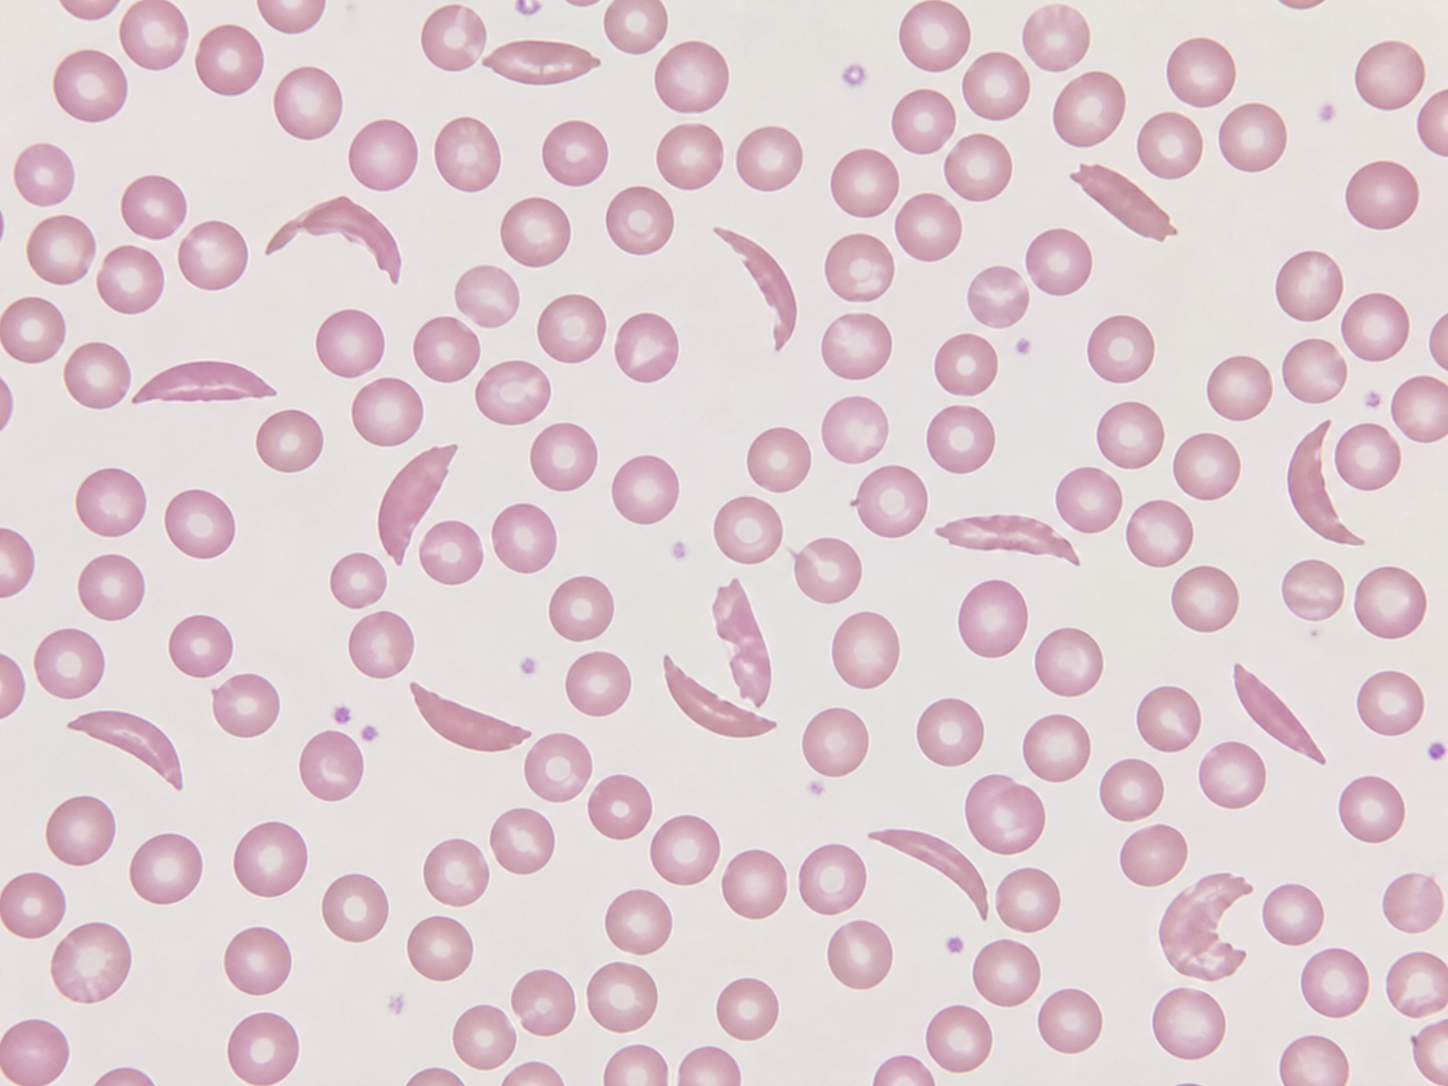
\includegraphics[width=0.56\linewidth]{images/book2/ai/g11-disease-sickle-smear.png}

{\small हँसिया-कोशिका रोग वाले किसी व्यक्ति का रक्त-लेप: गोल लाल \omterm{def:g10:cells-common-unit:cell}{कोशिकाएँ},
और उनके बीच वे हँसिये। दोनों विकल्पियों पर ढोए गए एक ही \omterm{def:g10:chemistry-of-life:families}{ऐमीनो अम्ल}
प्रतिस्थापन का कोशिकीय \omterm{def:g11:enzymes-and-phenotype:phenotype}{लक्षणप्ररूप}।}
\end{omfigure}

\section{कोई वंश-वृक्ष पढ़ना}

\begin{definition}[वंशावली]\label{def:g11:genes-and-disease:pedigree}
\emph{वंशावली}\index{वंशावली} कई पीढ़ियों तक किसी परिवार का आरेख है: पुरुषों
के लिए वर्ग, स्त्रियों के लिए वृत्त, किसी दंपती को जोड़ती एक क्षैतिज रेखा,
उनके बच्चों तक जाती एक ऊर्ध्वाधर रेखा, और रोगग्रस्त लोगों के लिए भरे हुए
चिह्न। पीढ़ियाँ ऊपर से I, II, III गिनी जाती हैं; और व्यक्ति बाएँ से गिने
जाते हैं।
\end{definition}

\begin{omfigure}
\begin{tikzpicture}[font=\small, line cap=round]
  \tikzset{m/.style={draw, thick, minimum size=0.5cm, inner sep=0},
           f/.style={draw, thick, circle, minimum size=0.5cm, inner sep=0},
           aff/.style={fill=omThm!70}}
  % generation I
  \node[m] (I1) at (2,3) {}; \node[f] (I2) at (3.2,3) {};
  \node[m] (I3) at (6.4,3) {}; \node[f] (I4) at (7.6,3) {};
  \draw[thick] (I1) -- (I2); \draw[thick] (I3) -- (I4);
  \node[anchor=east] at (0.8,3) {I};
  \foreach \n/\x in {1/2, 2/3.2, 3/6.4, 4/7.6} \node[font=\scriptsize, anchor=south] at (\x,3.35) {\n};
  % generation II
  \draw[thick] (2.6,3) -- (2.6,2.3) -- (4.4,2.3); \draw[thick] (1.6,2.3) -- (2.6,2.3);
  \draw[thick] (7.0,3) -- (7.0,2.3) -- (5.6,2.3); \draw[thick] (7.0,2.3) -- (8.4,2.3);
  \node[f] (II1) at (1.6,1.7) {}; \node[m, aff] (II2) at (2.6,1.7) {}; \node[m] (II3) at (4.4,1.7) {};
  \node[f] (II4) at (5.6,1.7) {}; \node[f] (II5) at (7.0,1.7) {}; \node[m] (II6) at (8.4,1.7) {};
  \foreach \x in {1.6,2.6,4.4,5.6,7.0,8.4} \draw[thick] (\x,2.3) -- (\x,1.95);
  \draw[thick] (II3) -- (II4);
  \node[anchor=east] at (0.8,1.7) {II};
  \foreach \n/\x in {1/1.6, 2/2.6, 3/4.4, 4/5.6, 5/7.0, 6/8.4} \node[font=\scriptsize, anchor=north] at (\x,1.42) {\n};
  % generation III
  \draw[thick] (5.0,1.7) -- (5.0,1.0) -- (5.8,1.0); \draw[thick] (4.2,1.0) -- (5.0,1.0);
  \node[m] (III1) at (4.2,0.4) {}; \node[f, aff] (III2) at (5.8,0.4) {};
  \foreach \x in {4.2,5.8} \draw[thick] (\x,1.0) -- (\x,0.65);
  \node[anchor=east] at (0.8,0.4) {III};
  \foreach \n/\x in {1/4.2, 2/5.8} \node[font=\scriptsize, anchor=north] at (\x,0.12) {\n};
  % legend
  \node[m] at (10.2,2.6) {}; \node[anchor=west] at (10.5,2.6) {पुरुष};
  \node[f] at (10.2,1.9) {}; \node[anchor=west] at (10.5,1.9) {स्त्री};
  \node[m, aff] at (10.2,1.2) {}; \node[anchor=west] at (10.5,1.2) {रोगग्रस्त};
\end{tikzpicture}

{\small सिस्टिक फ़ाइब्रोसिस के लिए एक \omterm{def:g11:genes-and-disease:pedigree}{वंशावली}। II-2 और III-2 रोगग्रस्त
हैं; उनके माता-पिता स्वस्थ हैं। इसलिए I-1/I-2 और II-3/II-4, दोनों दंपती
वाहक ही होंगे; और II-3, जो किसी रोगग्रस्त बच्चे का स्वस्थ भाई है,
$2/3$ प्रायिकता से वाहक है।}
\end{omfigure}

\begin{method}[किसी वंशावली का विश्लेषण]\label{met:g11:genes-and-disease:analyse}
\begin{enumerate}
  \item \emph{\omterm{def:g11:genes-and-disease:genetic}{प्रभावी} या \omterm{def:g11:genes-and-disease:genetic}{अप्रभावी}?} दो स्वस्थ माता-पिता का रोगग्रस्त
        बच्चा \omterm{def:g11:genes-and-disease:genetic}{अप्रभावी} का मतलब है (माता-पिता वाहक हैं)। और हर पीढ़ी में
        रोगग्रस्त जनक वाला रोगग्रस्त व्यक्ति \omterm{def:g11:genes-and-disease:genetic}{प्रभावी} का संकेत देता है।
  \item \emph{किसी लिंग \omterm{def:g11:cell-cycle-mitosis:chromosome}{गुणसूत्र} पर?} यदि केवल पुरुष रोगग्रस्त हों और
        उनकी माताओं के भाई या पिता भी हों, तो X \omterm{def:g11:cell-cycle-mitosis:chromosome}{गुणसूत्र} का शक कीजिए
        (नीचे)। वरना वह \omterm{def:g10:universal-dna:gene}{जीन} किसी साधारण \omterm{def:g11:cell-cycle-mitosis:chromosome}{गुणसूत्र} पर है।
  \item \emph{\omterm{def:g11:enzymes-and-phenotype:phenotype}{जीनप्ररूप} सौंपिए}: किसी \omterm{def:g11:genes-and-disease:genetic}{अप्रभावी} रोग में रोगग्रस्त लोग $aa$
        हैं; उनके माता-पिता और बच्चे कम से कम एक $a$ ढोते हैं; और किसी
        रोगग्रस्त के स्वस्थ सहोदर $AA$ या $Aa$ हैं।
  \item \emph{जोखिम निकालिए}: किसी सोचे हुए बच्चे के लिए माता-पिता के
        \omterm{def:g11:enzymes-and-phenotype:phenotype}{जीनप्ररूप} किसी पुनेट वर्ग में मिलाइए; और जब किसी जनक का \omterm{def:g11:enzymes-and-phenotype:phenotype}{जीनप्ररूप}
        अनिश्चित हो, तो हर संभावना को उसकी प्रायिकता से तौलिए।
\end{enumerate}
\end{method}

\begin{example}[वे दो-तिहाई]\label{ex:g11:genes-and-disease:twothirds}
किसी रोगग्रस्त बच्चे का स्वस्थ भाई $2/3$ प्रायिकता से वाहक क्यों है,
$1/2$ से क्यों नहीं? माता-पिता $Aa \times Aa$ हैं; और कोई बच्चा बराबर संभावनाओं
से $AA$, $Aa$, $aA$ या $aa$ है। वह स्वस्थ है, यह जान लेने से $aa$ हट जाता
है: तीन हाल बचते हैं, जिनमें से दो वाहक हैं। यदि वह आम आबादी की किसी
स्त्री से विवाह करे (जो $1/25$ प्रायिकता से वाहक है), तो पहले बच्चे के
रोगग्रस्त होने का जोखिम
$2/3 \times 1/25 \times 1/4 = 1/150$ है।
\end{example}

\section{X गुणसूत्र के जीन}

\begin{proposition}[X-सहलग्न वंशागति]\label{prop:g11:genes-and-disease:xlinked}
स्त्रियाँ दो X \omterm{def:g11:cell-cycle-mitosis:chromosome}{गुणसूत्र} ढोती हैं, और पुरुष एक X तथा एक Y। X \omterm{def:g11:cell-cycle-mitosis:chromosome}{गुणसूत्र} पर का
कोई \omterm{def:g11:genes-and-disease:genetic}{अप्रभावी} \omterm{def:g10:universal-dna:gene}{युग्मविकल्पी} किसी स्त्री में उसके दूसरे X से ढँक जाता है, पर कोई
पुरुष, जिसके पास दूसरा X है ही नहीं, उसे व्यक्त कर देता है। इसलिए ऐसा रोग
ज़्यादातर पुरुषों को होता है; किसी रोगग्रस्त पुरुष की सारी बेटियाँ वाहक
होती हैं; और कोई वाहक माता वह \omterm{def:g10:universal-dna:gene}{युग्मविकल्पी} अपने आधे बेटों को देती है, जो
रोगग्रस्त होते हैं, तथा आधी बेटियों को, जो वाहक होती हैं। हीमोफ़ीलिया,
जिसमें रक्त जम ही नहीं पाता, इसका जाना-पहचाना उदाहरण है; और लाल-हरा
वर्णांधता (\cref{ch:g11:the-eye}) दूसरा।
\end{proposition}
\admitted

\begin{omfigure}
\begin{tikzpicture}[font=\small]
  \draw[thick] (0,0) grid[step=2.2] (4.4,4.4);
  \node[anchor=south] at (1.1,4.5) {$X^H$}; \node[anchor=south] at (3.3,4.5) {$Y$};
  \node[anchor=east] at (-0.15,3.3) {$X^H$}; \node[anchor=east] at (-0.15,1.1) {$X^h$};
  \node[anchor=south, font=\small\itshape] at (2.2,5.0) {पिता (स्वस्थ)};
  \node[font=\small\itshape, rotate=90, anchor=south] at (-0.95,2.2) {माता (वाहक)};
  \node[fill=omDef!15, minimum size=2.1cm, align=center, font=\footnotesize] at (1.1,3.3) {$X^HX^H$\\ स्वस्थ लड़की};
  \node[fill=omDef!15, minimum size=2.1cm, align=center, font=\footnotesize] at (3.3,3.3) {$X^HY$\\ स्वस्थ लड़का};
  \node[fill=omProp!20, minimum size=2.1cm, align=center, font=\footnotesize] at (1.1,1.1) {$X^HX^h$\\ वाहक लड़की};
  \node[fill=omThm!25, minimum size=2.1cm, align=center, font=\footnotesize] at (3.3,1.1) {$X^hY$\\ रोगग्रस्त लड़का};
  \node[anchor=west, align=left, text width=6cm] at (5.4,2.2) {वाहक माता और स्वस्थ पिता: आधे बेटे रोगग्रस्त, आधी बेटियाँ वाहक, और कोई रोगग्रस्त बेटी नहीं। $Y$ उस जीन की कोई प्रति नहीं ढोता, इसलिए किसी बेटे की अकेली प्रति उसकी माता से ही आती है।};
\end{tikzpicture}

{\small हीमोफ़ीलिया जैसे किसी X-सहलग्न \omterm{def:g11:genes-and-disease:genetic}{अप्रभावी} रोग के लिए पुनेट वर्ग
($h$, यानी उत्परिवर्ती \omterm{def:g10:universal-dna:gene}{युग्मविकल्पी}; $H$, यानी साधारण वाला)।}
\end{omfigure}

\section{ख़ुद जीन को पढ़ना}

\begin{proposition}[आनुवंशिक जाँच]\label{prop:g11:genes-and-disease:testing}
कोई व्यक्ति जो \omterm{def:g10:universal-dna:gene}{युग्मविकल्पी} ढोता है वे उसके \omterm{def:g10:universal-dna:information}{DNA} से सीधे पढ़े जा सकते हैं, जो चंद
\omterm{def:g10:cells-common-unit:cell}{कोशिकाओं} से निकाला जाता है (रक्त, लार, और किसी गर्भस्थ शिशु के लिए नाल का
या उसके चारों ओर के तरल का नमूना)। उस \omterm{def:g10:universal-dna:gene}{जीन} का क्षेत्र किसी ऐसी अभिक्रिया से
लाखों बार नक़ल किया जाता है जो परखनली में प्रतिकृतिकरण की नक़ल करती है
(\cref{ch:g11:dna-replication}), और फिर या तो उसका अनुक्रमण होता है या उसे
विशिष्ट अनुक्रम पहचानने वाले \omterm{def:g11:enzymes-and-phenotype:enzyme}{एंजाइम} काट देते हैं और उन्हें जेल में आकार के
हिसाब से छाँटा जाता है: जिस उत्परिवर्ती \omterm{def:g10:universal-dna:gene}{युग्मविकल्पी} ने कोई कटान-स्थल पाया,
खोया या बदला हो वह अलग लंबाइयों के टुकड़े देता है, जो पट्टियों के रूप में
दिखते हैं। ऐसी जाँचें किसी बच्चे के गर्भ में आने से पहले ही वाहक पहचान लेती
हैं, गर्भस्थ शिशु का निदान करती हैं, और लक्षण उभरने से पहले किसी नवजात में
उस \omterm{def:g11:mutations:mutation}{उत्परिवर्तन} का पता लगा लेती हैं।
\end{proposition}
\admitted

\begin{omfigure}
\begin{tikzpicture}[font=\small]
  % gel: 4 lanes
  \fill[gray!15] (0,0) rectangle (7.2,4.2);
  \foreach \x/\l in {0.9/{आकार की\\ सीढ़ी}, 2.7/{$AA$}, 4.5/{$Aa$}, 6.3/{$aa$}} \node[anchor=south, align=center] at (\x,4.3) {\l};
  % ladder
  \foreach \y in {3.6,3.1,2.6,2.0,1.4,0.8} \fill[omDef!70] (0.5,\y) rectangle (1.3,\y+0.1);
  % AA: one band (600 bp, cut into 400+200? keep: A allele = one long fragment at 3.1)
  \fill[omThm!80] (2.3,3.1) rectangle (3.1,3.2);
  % Aa: long fragment + two short
  \fill[omThm!80] (4.1,3.1) rectangle (4.9,3.2);
  \fill[omThm!80] (4.1,2.0) rectangle (4.9,2.1);
  \fill[omThm!80] (4.1,1.4) rectangle (4.9,1.5);
  % aa: two short only
  \fill[omThm!80] (5.9,2.0) rectangle (6.7,2.1);
  \fill[omThm!80] (5.9,1.4) rectangle (6.7,1.5);
  \draw[->, thick] (7.6,3.8) -- (7.6,0.8) node[midway, right, align=left] {प्रवास की\\ दिशा:\\ छोटे टुकड़े\\ अधिक दूर जाते हैं};
  \node[anchor=east, font=\scriptsize] at (0.4,3.15) {600 जोड़े};
  \node[anchor=east, font=\scriptsize] at (0.4,2.05) {400 जोड़े};
  \node[anchor=east, font=\scriptsize] at (0.4,1.45) {200 जोड़े};
\end{tikzpicture}

{\small जेल पर \omterm{def:g10:universal-dna:gene}{युग्मविकल्पी} पढ़ना। उत्परिवर्ती \omterm{def:g10:universal-dna:gene}{युग्मविकल्पी} $a$ ने एक कटान-स्थल पा
लिया है: इसलिए $A$ का 600 क्षारक-जोड़ों वाला टुकड़ा कटकर 400 और 200 बन जाता
है। कोई वाहक तीनों पट्टियाँ दिखाता है; और कोई रोगग्रस्त केवल दोनों छोटी।}
\end{omfigure}

\begin{omfigure}
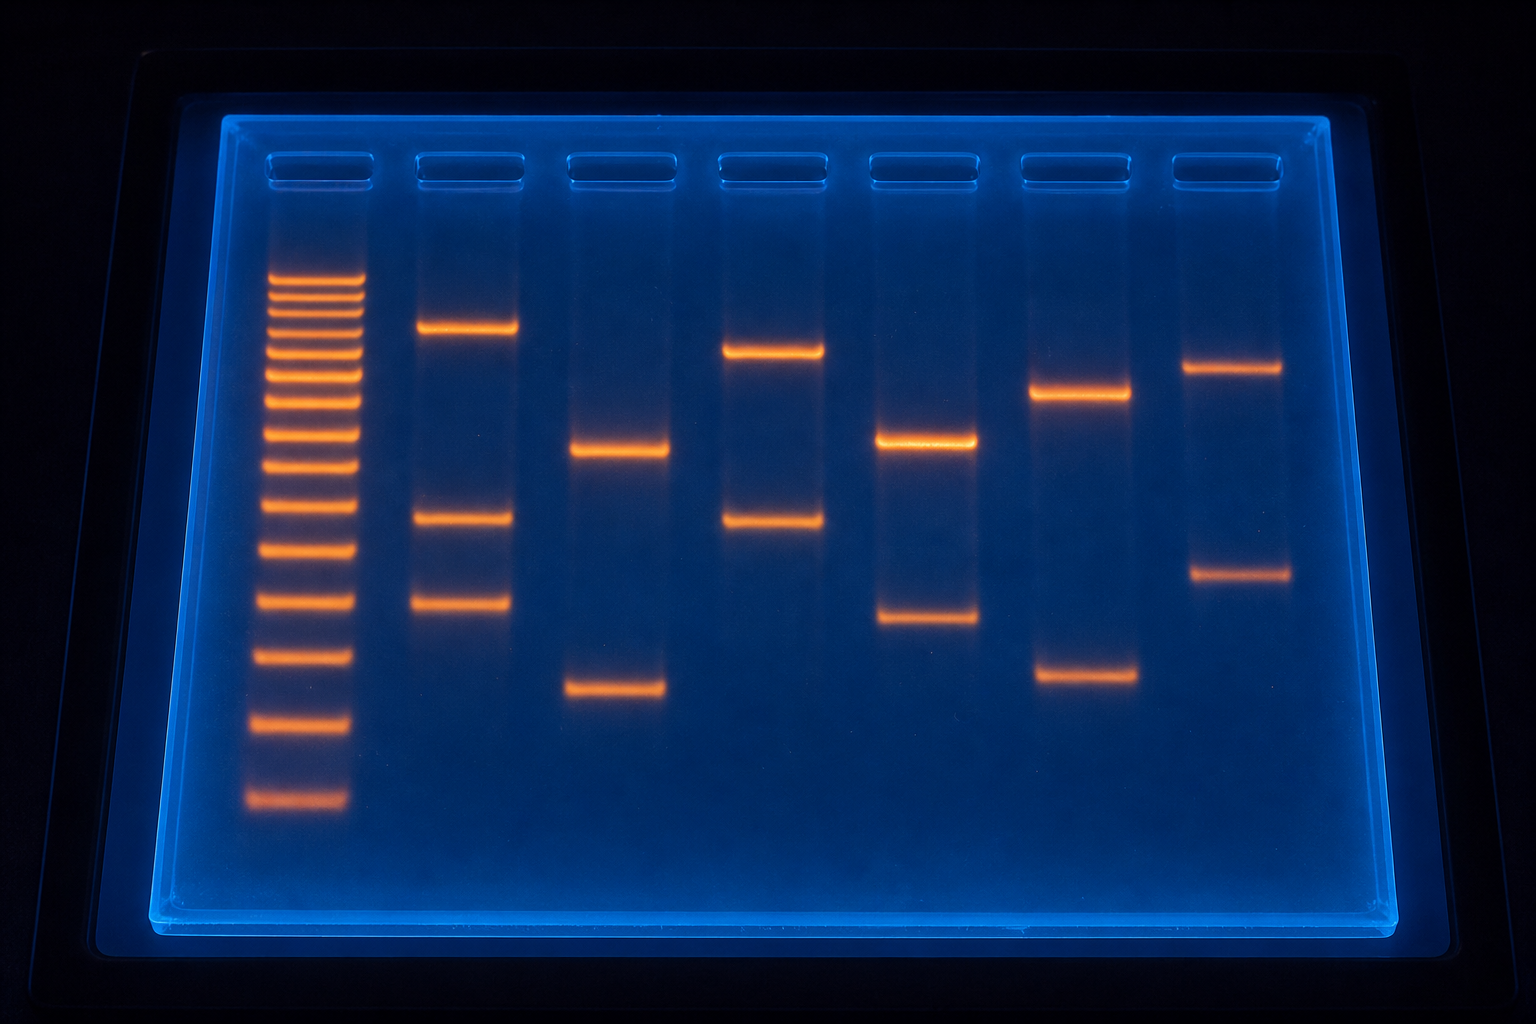
\includegraphics[width=0.56\linewidth]{images/book2/ai/g11-disease-gel.png}

{\small पराबैंगनी प्रकाश के नीचे वैद्युतकणसंचलन का एक जेल: प्रतिदीप्त रंगे
हुए \omterm{def:g10:universal-dna:information}{DNA} टुकड़े, लंबाई के हिसाब से छँटे हुए। हर लेन एक नमूना है; और पट्टियों
का ढर्रा \omterm{def:g10:universal-dna:gene}{युग्मविकल्पी} पढ़ देता है।}
\end{omfigure}

\begin{example}[कोई जाँच क्या कह सकती है और क्या नहीं]\label{ex:g11:genes-and-disease:testsays}
सिस्टिक फ़ाइब्रोसिस की वाहक-जाँच पचास सबसे आम उत्परिवर्ती \omterm{def:g10:universal-dna:gene}{युग्मविकल्पी} ढूँढ़ती है
और लगभग 90\% वाहक पकड़ लेती है: इसलिए ऋणात्मक नतीजा किसी व्यक्ति के वाहक
होने की संभावना $1/25$ से घटाकर लगभग $1/250$ कर देता है, पर उसे शून्य नहीं
करता। दो ज्ञात वाहकों के गर्भस्थ शिशु का जन्मपूर्व निदान लगभग निश्चित होता
है, और माता-पिता के सामने ऐसा फ़ैसला खड़ा कर देता है जो जीवविज्ञान उनके लिए
नहीं करता। और हंटिंगटन रोग की जाँच किसी स्वस्थ तीस-वर्षीय को बता देती है कि
वह रोग आएगा या नहीं; पर जिन्हें उसका हक़ है उनमें से एक-तिहाई न जानना ही
चुनते हैं।
\end{example}

\section{बहुत-से जीनों के और जीने के ढंग के रोग}

\begin{proposition}[बहुकारकीय रोग]\label{prop:g11:genes-and-disease:multifactorial}
अधिकांश आम रोग --- टाइप 2 मधुमेह, हृदय और धमनी के रोग, अधिकांश कैंसर, दमा
--- \emph{बहुकारकीय}\index{बहुकारकीय रोग} हैं: दर्जनों या सैकड़ों \omterm{def:g10:universal-dna:gene}{युग्मविकल्पी}
जोखिम को थोड़ा-थोड़ा खिसकाते हैं, और पर्यावरण (आहार, क्रिया, धूम्रपान,
संक्रमण) उसे बहुत खिसका देता है। ऐसा रोग परिवारों में चलता तो है पर किसी
एक \omterm{def:g10:universal-dna:gene}{जीन} के नियमों पर नहीं चलता, और कोई आनुवंशिक प्रवृत्ति एक जोखिम है, कोई
सज़ा नहीं: वही \omterm{def:g10:universal-dna:gene}{युग्मविकल्पी} जीने के एक ढंग में रोग देते हैं और दूसरे में नहीं।
\end{proposition}
\begin{proof}[साक्ष्य]
समरूप जुड़वाँ अपने सारे \omterm{def:g10:universal-dna:gene}{युग्मविकल्पी} साझा करते हैं; और जब उनमें से एक को टाइप 2
मधुमेह हो, तो लगभग 70\% हालों में दूसरे को भी होता है --- यानी आबादी के 8\%
से कहीं ऊपर, इसलिए \omterm{def:g10:universal-dna:gene}{जीन} मायने रखते हैं --- पर 100\% नहीं, इसलिए \omterm{def:g10:universal-dna:gene}{जीन} फ़ैसला
नहीं करते। जो आबादियाँ एक ही पीढ़ी में गाँव के आहार से शहरी आहार पर आ गईं,
उनमें उन्हीं \omterm{def:g10:universal-dna:gene}{जीनों} के साथ यह रोग कई गुना बढ़ गया। और बहुत-से जोखिम \omterm{def:g10:universal-dna:gene}{युग्मविकल्पी}
ढोते लोगों में जो सक्रिय तथा दुबले रहते हैं उनमें यह रोग बाक़ियों की दर के
एक अंश भर पर ही होता है।
\end{proof}

\begin{omfigure}
\begin{tikzpicture}
\begin{axis}[
  ybar, bar width=12pt,
  width=0.8\linewidth, height=5.4cm,
  axis x line=bottom, axis y line=left,
  ymin=0, ymax=40, ylabel={60 की उम्र तक टाइप 2 मधुमेह (\%)},
  ylabel style={font=\small},
  symbolic x coords={थोड़े जोखिम युग्मविकल्पी, औसत, बहुत जोखिम युग्मविकल्पी},
  xtick=data, tick label style={font=\small},
  enlarge x limits=0.25, ytick={0,10,20,30,40},
  legend style={at={(0.5,-0.2)}, anchor=north, legend columns=2, font=\small, draw=none},
  nodes near coords, nodes near coords style={font=\scriptsize},
]
\addplot[fill=omMeth!50, draw=omMeth] coordinates {(थोड़े जोखिम युग्मविकल्पी,3) (औसत,6) (बहुत जोखिम युग्मविकल्पी,12)};
\addplot[fill=omThm!50, draw=omThm] coordinates {(थोड़े जोखिम युग्मविकल्पी,9) (औसत,17) (बहुत जोखिम युग्मविकल्पी,34)};
\legend{सक्रिय और दुबले, गतिहीन और अधिक वज़नी}
\end{axis}
\end{tikzpicture}

{\small आनुवंशिक अंक और जीने के ढंग के हिसाब से टाइप 2 मधुमेह का जोखिम
(आबादी के अध्ययनों से गोल किया हुआ)। \omterm{def:g10:universal-dna:gene}{जीन} पैमाने के एक सिरे से दूसरे तक
जोखिम चार गुना कर देते हैं; और जीने का ढंग उसे पैमाने के हर बिंदु पर तीन
गुना। दोनों साथ मिलकर काम करते हैं।}
\end{omfigure}

\begin{remark}[तो फिर ``आनुवंशिक'' का अर्थ क्या है]\label{rem:g11:genes-and-disease:meaning}
सिस्टिक फ़ाइब्रोसिस कड़े अर्थ में आनुवंशिक है: \omterm{def:g11:enzymes-and-phenotype:phenotype}{जीनप्ररूप} ही वह रोग तय करता
है, पर्यावरण चाहे जो हो, और पर्यावरण केवल यह बदलता है कि उसे जिया कैसे
जाए। टाइप 2 मधुमेह किसी कमज़ोर अर्थ में आनुवंशिक है: \omterm{def:g11:enzymes-and-phenotype:phenotype}{जीनप्ररूप} एक
सुग्राहिता तय करता है, जिसे पर्यावरण सच करता है या नहीं। इन दोनों के बीच
फेनिलकीटोनूरिया आता है, जहाँ कोई आहार \omterm{def:g11:enzymes-and-phenotype:phenotype}{जीनप्ररूप} का असर रद्द कर देता है, और
हँसिया-कोशिका का वाहक, जिसका \omterm{def:g10:universal-dna:gene}{युग्मविकल्पी} एक जगह रोग है और दूसरी जगह बचाव।
``क्या यह आनुवंशिक है?'' शायद ही कभी हाँ-या-ना का सवाल होता है; पूछने लायक़
सवाल है ``कितना, और किन शर्तों में?''
\end{remark}

\section{अभ्यास}

\begin{exercise}[$\star$]\label{exo:g11:genes-and-disease:1}
\omterm{def:g11:genes-and-disease:genetic}{अप्रभावी} और \omterm{def:g11:genes-and-disease:genetic}{प्रभावी} \omterm{def:g10:universal-dna:gene}{युग्मविकल्पी} तथा वाहक की परिभाषा दीजिए।
\end{exercise}

\begin{exercise}[$\star$]\label{exo:g11:genes-and-disease:2}
सिस्टिक फ़ाइब्रोसिस के दो वाहकों के यहाँ एक बच्चा होता है। बच्चे के
रोगग्रस्त होने, वाहक होने, या इनमें से कुछ न होने की प्रायिकता बताइए।
\end{exercise}

\begin{exercise}[$\star$]\label{exo:g11:genes-and-disease:3}
\omterm{def:g11:genes-and-disease:pedigree}{वंशावली} वाले चित्र में I-1, I-2, II-2 और III-2 के \omterm{def:g11:enzymes-and-phenotype:phenotype}{जीनप्ररूप} बताइए।
\end{exercise}

\begin{exercise}[$\star$]\label{exo:g11:genes-and-disease:4}
X-सहलग्न \omterm{def:g11:genes-and-disease:genetic}{अप्रभावी} रोग पुरुषों में कहीं अधिक आम क्यों हैं?
\end{exercise}

\begin{exercise}[$\star$]\label{exo:g11:genes-and-disease:5}
\omterm{prop:g11:genes-and-disease:multifactorial}{बहुकारकीय रोग} क्या है? दो उदाहरण दीजिए।
\end{exercise}

\begin{exercise}[$\star\star$]\label{exo:g11:genes-and-disease:6}
सिस्टिक फ़ाइब्रोसिस वाला कोई व्यक्ति किसी बिना वाहक वाले से विवाह करता है।
उनके बच्चे कैसे होंगे? और उनमें से किसी के, किसी वाहक के साथ, बच्चे?
\end{exercise}

\begin{exercise}[$\star\star$]\label{exo:g11:genes-and-disease:7}
\omterm{def:g11:genes-and-disease:pedigree}{वंशावली} वाले चित्र में II-1 के वाहक होने की प्रायिकता निकालिए, और II-1
तथा आम आबादी के किसी पुरुष के बच्चे के रोगग्रस्त होने की प्रायिकता भी।
\end{exercise}

\begin{exercise}[$\star\star$]\label{exo:g11:genes-and-disease:8}
हंटिंगटन रोग (\omterm{def:g11:genes-and-disease:genetic}{प्रभावी}, एक उत्परिवर्ती \omterm{def:g10:universal-dna:gene}{युग्मविकल्पी}) वाले किसी पुरुष और किसी
स्वस्थ स्त्री के चार बच्चे हैं। किसी दिए हुए बच्चे को वह रोग विरासत में
मिलने की प्रायिकता क्या है? और चारों में से किसी को भी न मिलने की?
\end{exercise}

\begin{exercise}[$\star\star$]\label{exo:g11:genes-and-disease:9}
कोई हीमोफ़ीलिया वाला पुरुष किसी बिना वाहक वाली स्त्री से विवाह करता है।
उनके बच्चों के \omterm{def:g11:enzymes-and-phenotype:phenotype}{जीनप्ररूप} तथा \omterm{def:g11:enzymes-and-phenotype:phenotype}{लक्षणप्ररूप} बताइए, और किसी स्वस्थ पुरुष से
विवाहित बेटी के ज़रिए नातियों-पोतों के भी।
\end{exercise}

\begin{exercise}[$\star\star$]\label{exo:g11:genes-and-disease:10}
जेल वाले चित्र में ऐसा व्यक्ति कौन-सी पट्टियाँ दिखाता जो दो अलग-अलग
उत्परिवर्ती \omterm{def:g10:universal-dna:gene}{युग्मविकल्पी} ढोता हो, जिनमें से एक कटान-स्थल जोड़ता हो और दूसरा 400
वाले टुकड़े से 100 क्षारक-जोड़े और हटा देता हो?
\end{exercise}

\begin{exercise}[$\star\star$]\label{exo:g11:genes-and-disease:11}
समझाइए कि \omterm{def:g11:mutations:mutation}{उत्परिवर्तन} की दर एक ही होते हुए भी सिस्टिक फ़ाइब्रोसिस यूरोप में
पूर्वी एशिया से हज़ार गुना आम क्यों है।
\end{exercise}

\begin{exercise}[$\star\star\star$]\label{exo:g11:genes-and-disease:12}
किसी दंपती के पहले बच्चे को सिस्टिक फ़ाइब्रोसिस है। दूसरे के रोगग्रस्त होने
की प्रायिकता निकालिए, फिर अगले दो में से कम से कम एक के। समझाइए कि
``हमारा चार में से एक हो चुका'' एक भ्रम क्यों है।
\end{exercise}

\begin{exercise}[$\star\star\star$]\label{exo:g11:genes-and-disease:13}
कोई वाहक-जाँच 90\% उत्परिवर्ती \omterm{def:g10:universal-dna:gene}{युग्मविकल्पी} पकड़ती है। आम आबादी की किसी स्त्री
की जाँच ऋणात्मक आती है। उसके वाहक होने की बची हुई प्रायिकता निकालिए, और
किसी ज्ञात वाहक साथी के साथ रोगग्रस्त बच्चे का जोखिम भी।
\end{exercise}

\begin{exercise}[$\star\star\star$]\label{exo:g11:genes-and-disease:14}
मधुमेह वाले चित्र से, बहुत-से जोखिम \omterm{def:g10:universal-dna:gene}{युग्मविकल्पी} ढोते किसी व्यक्ति के लिए
``बहुत'' से ``थोड़े'' जोखिम विकल्पियों पर जाने (जो असंभव है) के असर की
तुलना गतिहीन से सक्रिय होने (जो संभव है) के असर से कीजिए। किसी आनुवंशिक
जोखिम-अंक का इस्तेमाल किसलिए होना चाहिए?
\end{exercise}

\begin{exercise}[$\star\star\star$]\label{exo:g11:genes-and-disease:15}
एक अनुच्छेद में चर्चा कीजिए कि हंटिंगटन रोग की जाँच किसी ऐसे स्वस्थ युवा
वयस्क को, जिसका कोई जनक रोगग्रस्त है, क्या देती है और क्या लेती है, और वह
फ़ैसला उसी का क्यों है।
\end{exercise}

\section{समस्या: एक परिवार, एक जीन}

\begin{problem}[{सप्ताहांत समस्या --- सिस्टिक फ़ाइब्रोसिस वाले एक परिवार का
तीन पीढ़ियों तक पीछा: जीनप्ररूप सौंपे गए, हर सोचे हुए बच्चे के लिए जोखिम
निकाले गए, प्रयोगशाला की एक जाँच पढ़ी गई, और वाहकों की आबादी का गणित}]
\label{pb:g11:genes-and-disease:1}
लिया और टॉम, दोनों स्वस्थ, के तीन बच्चे हैं: मैक्स (स्वस्थ), ज़ोए (सिस्टिक
फ़ाइब्रोसिस) और लू (स्वस्थ)। टॉम की बहन आना स्वस्थ है और करीम से विवाहित,
जिसके परिवार में इस रोग का कोई इतिहास नहीं; वे एक बच्चे की उम्मीद कर रहे
हैं। आबादी में 25 में एक व्यक्ति वाहक है।

\medskip
\noindent\textbf{भाग I --- \omterm{def:g11:enzymes-and-phenotype:phenotype}{जीनप्ररूप}।}
\begin{enumerate}
  \item यह रोग \omterm{def:g11:genes-and-disease:genetic}{प्रभावी} है या \omterm{def:g11:genes-and-disease:genetic}{अप्रभावी}? परिवार से कारण बताइए।
  \item लिया, टॉम और ज़ोए के \omterm{def:g11:enzymes-and-phenotype:phenotype}{जीनप्ररूप} बताइए।
  \item मैक्स के संभव \omterm{def:g11:enzymes-and-phenotype:phenotype}{जीनप्ररूप} क्या हैं, और किन-किन प्रायिकताओं के साथ?
  \item आना के वाहक होने की प्रायिकता क्या है? (उसके माता-पिता पर विचार
        कीजिए।)
  \item करीम के वाहक होने की प्रायिकता क्या है?
\end{enumerate}

\medskip
\noindent\textbf{भाग II --- जोखिम।}
\begin{enumerate}[resume]
  \item आना और करीम के बच्चे के रोगग्रस्त होने की प्रायिकता निकालिए।
  \item लिया और टॉम चौथे बच्चे पर विचार कर रहे हैं। उसके रोगग्रस्त होने
        की प्रायिकता? और वाहक होने की?
  \item वयस्क मैक्स आम आबादी की किसी स्त्री से विवाह करता है। पहले बच्चे
        के रोगग्रस्त होने की प्रायिकता?
  \item वयस्क ज़ोए आम आबादी के किसी पुरुष से विवाह करती है। बच्चे के
        रोगग्रस्त होने की प्रायिकता? और वाहक होने की?
  \item लू आना और करीम के किसी बच्चे, यानी अपने चचेरे भाई-बहन, से विवाह
        करती है। रोगग्रस्त बच्चे की प्रायिकता निकालिए। वह मैक्स के
        मुक़ाबले अधिक क्यों है?
\end{enumerate}

\medskip
\noindent\textbf{भाग III --- जाँच।}
इस परिवार में ढोया जाने वाला उत्परिवर्ती \omterm{def:g10:universal-dna:gene}{युग्मविकल्पी} एक कटान-स्थल जोड़ देता है:
साधारण \omterm{def:g10:universal-dna:gene}{युग्मविकल्पी} 900 क्षारक-जोड़ों का एक टुकड़ा देता है, और उत्परिवर्ती 600
तथा 300 के।
\begin{enumerate}[resume]
  \item ज़ोए के लिए, टॉम के लिए और किसी बिना वाहक वाले के लिए अपेक्षित
        पट्टियाँ खींचिए या उनका वर्णन कीजिए।
  \item मैक्स की जाँच होती है: 900 पर एक पट्टी। अब उसका \omterm{def:g11:enzymes-and-phenotype:phenotype}{जीनप्ररूप} क्या है,
        और उसके पहले बच्चे के लिए नया जोखिम (प्रश्न 8) क्या है?
  \item आना की जाँच होती है: 900, 600 और 300 पर पट्टियाँ। उसके बच्चे के
        लिए जोखिम दोबारा निकालिए।
  \item करीम की जाँच में पचास सबसे आम उत्परिवर्ती विकल्पियों में से कोई
        नहीं मिलता, और वे 90\% वाहक ढँकते हैं। उसके वाहक होने की बची हुई
        प्रायिकता निकालिए और जोखिम दोबारा निकालिए।
  \item आना और करीम के गर्भस्थ शिशु की जन्मपूर्व जाँच 900, 600 और 300 पर
        पट्टियाँ दिखाती है। उस शिशु का \omterm{def:g11:enzymes-and-phenotype:phenotype}{जीनप्ररूप} और \omterm{def:g11:enzymes-and-phenotype:phenotype}{लक्षणप्ररूप} क्या है?
\end{enumerate}

\medskip
\noindent\textbf{भाग IV --- आबादी।}
\begin{enumerate}[resume]
  \item यदि 25 में एक व्यक्ति वाहक हो, तो किसी यादृच्छिक दंपती के दोनों
        सदस्यों के वाहक होने की प्रायिकता क्या है, और इससे रोगग्रस्त
        नवजातों की बारंबारता क्या?
  \item देखी गई 2500 में एक से तुलना कीजिए। टिप्पणी कीजिए।
  \item पहले लगभग सारे रोगग्रस्त बचपन में ही मर जाते थे। स्वस्थ वाहकों की
        बनाम रोगग्रस्तों की ढोई गई प्रतियों की संख्या की मदद से समझाइए कि
        फिर भी वह उत्परिवर्ती \omterm{def:g10:universal-dna:gene}{युग्मविकल्पी} 50 प्रतियों में एक की बारंबारता पर
        क्यों बना रहा।
  \item अब इलाज अधिकांश रोगग्रस्तों को वयस्कता तक पहुँचने और बच्चे पैदा
        करने देते हैं। आने वाली पीढ़ियों में उस \omterm{def:g10:universal-dna:gene}{युग्मविकल्पी} की बारंबारता पर असर
        का, और उसके आकार का, अनुमान लगाइए।
  \item परिणाम लिखिए: दो वाहकों वाला चार में एक, किसी स्वस्थ सहोदर वाला
        तीन में दो, और इस परिवार के गणित में जेल ने क्या जोड़ा।
\end{enumerate}
\end{problem}
